x%%%%%%%%%%%%%%%%%%%%%%%%%%%%%%%%%%%%%%%%%%%%%%%%%%%%%%%%%%%%%%%%%%%%%%%%%%%%%%%
%%                                                                           %%
%%   Dr Derek Harter                                                         %%
%%   Profesor, Department of Computer Science                                %% 
%%   Texas A&M University - Commerce, USA                                    %%
%%                                                                           %%
%%%%%%%%%%%%%%%%%%%%%%%%%%%%%%%%%%%%%%%%%%%%%%%%%%%%%%%%%%%%%%%%%%%%%%%%%%%%%%%
%%%%     SETTING STARTS - DO NOT CHANGE Unless your TeX setting require so   %%
%%%%%%%%%%%%%%%%%%%%%%%%%%%%%%%%%%%%%%%%%%%%%%%%%%%%%%%%%%%%%%%%%%%%%%%%%%%%%%%
%%----------------------------------------------------------------------------------
% DO NOT Change this. It is the required setting letterpaper page, 11pt, onside print, book style
%%----------------------------------------------------------------------------------
\documentclass[letterpaper,11pt,oneside]{book}

%%-------------------------------------
%% Page margin settings - % half inch margin all sides (recommended)
%%-------------------------------------
\usepackage[margin=1.2in]{geometry} 

%%-------------------------------------
%% Font settings - % CM San or Ariel (recommended)
%%-------------------------------------
% Switch the following two line off: to revert back to default LaTex font (NOT recommended)
\usepackage{amsfonts}
\renewcommand*\familydefault{\sfdefault}

%%-------------------------------------
%% Math/Definition/Theorem/Algorithm packages settings 
%%-------------------------------------
\usepackage[cmex10]{amsmath}
\usepackage{amssymb}
\usepackage{amsthm}
\newtheorem{mydef}{Definition}
\newtheorem{mytherm}{Theorem}

%%-------------------------------------
%% Algorithms/Code Listing environment settings  - 
%% Please do not change these settings
%%-------------------------------------
\usepackage{algorithm}
\usepackage{algpseudocode}
\renewcommand{\algorithmicrequire}{\textbf{Input:}}
\renewcommand{\algorithmicensure}{\textbf{Output:}}
\usepackage[utf8]{inputenc}
\usepackage{listings}
\usepackage{xcolor}
\definecolor{codegreen}{rgb}{0,0.6,0.1}
\definecolor{codegray}{rgb}{0.5,0.5,0.5}
\definecolor{codeblue}{rgb}{0.10,0.00,1.00}
\definecolor{codepurple}{rgb}{0.58,0,0.82}
\definecolor{backcolour}{rgb}{1.0,1.0,1.0}

\lstdefinestyle{mystyle}{
    backgroundcolor=\color{backcolour},   
    commentstyle=\color{codegreen},
    keywordstyle=\color{codeblue},
    numberstyle=\tiny\color{codegray},
    stringstyle=\color{codepurple},
    basicstyle=\ttfamily\footnotesize,
    breakatwhitespace=false,         
    breaklines=true,                 
    captionpos=b,                        
    keepspaces=true,                 
    numbers=left,                    
    numbersep=5pt,                  
    showspaces=false,                
    showstringspaces=false,
    showtabs=false,                  
    tabsize=2,
    frame=none
}
\lstset{style=mystyle}

%%-------------------------------------
%% Graphics/Figures environment settings
%%-------------------------------------
\usepackage{graphicx}
\usepackage{subfigure}
\usepackage{caption}
\usepackage{lipsum}

%%-------------------------------------
%% Table environment settings
%%-------------------------------------
\usepackage{multirow}
\usepackage{rotating}
\usepackage{makecell}
\usepackage{booktabs}
%\usepackage{longtable,booktabs}

%%-------------------------------------
%% List of Abbreviations settings
%%-------------------------------------
\usepackage{enumitem}
\newlist{abbrv}{itemize}{1}
\setlist[abbrv,1]{label=,labelwidth=1in,align=parleft,itemsep=0.1\baselineskip,leftmargin=!}

%%-------------------------------------
%% Bibliography/References settings   - Harvard Style was used in this report
%%-------------------------------------
\usepackage[hidelinks]{hyperref}
\usepackage[comma,authoryear]{natbib}
\renewcommand{\bibname}{References} % DO NOT remove or switch of 

%%-------------------------------------
%% Appendix settings     
%%-------------------------------------
\usepackage[toc]{appendix}
%%%%%%%%%%%%%%%%%%%%%%%%%%%%%%%%%%%%%%%%%%%%%%%%%%%%%%%%%%%%%%%%%%%%%%%%%%%%%%%%%%%%%%%
%%%%                     SETTING ENDS                                            %%%%%%
%%%%%%%%%%%%%%%%%%%%%%%%%%%%%%%%%%%%%%%%%%%%%%%%%%%%%%%%%%%%%%%%%%%%%%%%%%%%%%%%%%%%%%%
\begin{document}

%    \captionsetup[figure]{margin=1.5cm,font=small,name={Figure},labelsep=colon}
  %  \captionsetup[table]{margin=1.5cm,font=small,name={Table},labelsep=colon}
    \SetLipsumDefault{1}
    
    \frontmatter
    
    \begin{titlepage}      
        \begin{center}
            
\includegraphics[width=3cm]{figures/tamuc-logo.png}\\[0.5cm]
            {\LARGE Texas A\&M University - Commerce\\[0.5cm]
            Department of Computer Science}\\[2cm]
			%{\color{blue} \rule{\textwidth}{1pt}}
			
			% -------------------------------
			% You need to edit some details here
			% -------------------------------  
            \linespread{1.2}\huge {
                %%%%%%%%%%%%%%%%%%%%%%%%%%%%
                %TODO: 1 TITLE of Your PROJECT 
                %%%%%%%%%%%%%%%%%%%%%%%%%%%%
                % chnage the following line                
                Automated Blood Cell Identification and Counting
            }
            \linespread{1}~\\[2cm]
			%{\color{blue} \rule{\textwidth}{1pt}}
            {\Large 
                %%%%%%%%%%%%%%%%%%%%%%%%%%%%
                %TODO: 2 YOUR NAME
                %%%%%%%%%%%%%%%%%%%%%%%%%%%%             
                % chnage the following line
                Sridevi Sowmya Grandhi
                % change end             
            }\\[1cm] 
            

            {\large 
                %%%%%%%%%%%%%%%%%%%%%%%%%%%%
                %TODO: 3 YOUR NAME Supervisor's name(s)
                %%%%%%%%%%%%%%%%%%%%%%%%%%%%             
                % change the following line                
                \emph{Supervisor:} Derek Harter, Ph.D.}\\[1cm] % if applicable
            
    		% PLEASE DO NOT CHANGE THIS TEXT %
            \large A report submitted in partial fulfilment of the requirements of\\Texas A\&M University - Commerce for the degree of\\ Master of Science in \textit{Computer Science}\\[0.3cm] 
            \vfill
            
            
            \today % Please update this date you can use \date{April 2020} for fixed date
        \end{center}
    \end{titlepage}
    
    
    % -------------------------------------------------------------------
    % Declaration
    % -------------------------------------------------------------------
    \newpage
    \thispagestyle{empty}
    \chapter*{\Large Declaration}
    % PLEASE CHANGE THIS TEXT EXCEPT YOUR NAME%
    % -------------------------------
    %TODO: PLEASE ONLY UPDATE HERE -- PLEASE WRITE YOUR NAME %    
    % ------------------------------- 
    I,
    %%%%%%%%%%%%%%%%%%%%%%%
     Sridevi Sowmya Grandhi, % Mandatory part
    %%%%%%%%%%%%%%%%%%%%%%%
    of the Department of Computer Science, Texas A\&M University - Commerce, confirm that this is my own work and figures, tables, equations, code snippets, artworks, and illustrations in this report are original and have not been taken from any other person's work, except where the works of others have been explicitly acknowledged, quoted, and referenced. I understand that if failing to do so will be considered a case of plagiarism. Plagiarism is a form of academic misconduct and will be penalised accordingly. \\
    
    %% Please delete as appropriate. 
    \noindent
    %%%%%%%%%%%%%%%%%%%%%%%%%%%%%%%%%%%%%%%%%%%%%%% 
    %TODO 1 Consent for example copy -  we will use 
    I give consent to a copy of my report being shared with future students as an exemplar. \\
    
    \noindent
    %%%%%%%%%%%%%%%%%%%%%%%%%%%%%%%%%%%%%%%%%%%%%%% 
    %TODO 2 Consent to let the report to use use by library for public use
    I give consent for my work to be made available more widely to members of TAMUC and public with interest in teaching, learning and research. 
    %%%%%%%%%%%%%%%%%%%%%%%%%%%%%%%%%%%%%%%%%%%%%%%
    ~\\[1cm]
    \begin{flushright}
	%------------------------------ 
	% change the following line
    %TODO: PLEASE UPDATE  Your Name  -------------------------------%
	Sridevi Sowmya Grandhi % Please change it to your name
    
    \today
    \end{flushright}

     
    % -------------------------------------------------------------------
    % Abstract and Acknowledgement
    % -------------------------------------------------------------------
    
    %Two resources useful for abstract writing.
% Guidance of how to write an abstract/summary provided by Nature: https://cbs.umn.edu/sites/cbs.umn.edu/files/public/downloads/Annotated_Nature_abstract.pdf %https://writingcenter.gmu.edu/guides/writing-an-abstract
\chapter*{\center \Large  Abstract}
%%%%%%%%%%%%%%%%%%%%%%%%%%%%%%%%%%%%%%
% Replace all text with your text
%%%%%%%%%%%%%%%%%%%%%%%%%%%%%%%%%%%

In our cutting-edge approach to automate the identification and counting of three blood cell 
types, we employ a sophisticated fusion of deep learning and advanced image processing 
techniques, particularly focusing on object detection. Traditional complete blood cell counts 
necessitate laborious manual counting using a haemocytometer, involving intricate laboratory 
equipment and chemical compounds. This antiquated method is both time-consuming and burdensome. 
Our innovative solution utilizes Convolutional Neural Networks (CNNs) for intricate feature 
extraction from microscopic blood sample images. Incorporating state-of-the-art object 
detection algorithms, such as YOLO (You Only Look Once) or Faster R-CNN (Region-based 
Convolutional Neural Network), our system precisely identifies and localizes individual blood 
cells, overcoming the limitations of manual counting. Image processing techniques, including 
contrast enhancement and morphological operations, are strategically applied to optimize image 
quality and facilitate accurate object segmentation. This synergistic blend of deep learning 
and image processing not only expedites the diagnostic process but also significantly improves 
the accuracy and efficiency of blood cell identification and counting. By automating this 
intricate task, our approach aims to revolutionize medical diagnostics, providing healthcare 
professionals with a rapid and reliable tool for comprehensive blood cell analysis.

%%%%%%%%%%%%%%%%%%%%%%%%%%%%%%%%%%%%%%%%%%%%%%%%%%%%%%%%%%%%%%%%%%%%%%%%%s
~\\[1cm]
\noindent % Provide your key words
\textbf{Keywords:} a maximum of five keywords/keyphrase separated by commas

\vfill
\noindent



    % -------------------------------------------------------------------
	% Acknowledgement
	% -------------------------------------------------------------------
   
    \chapter*{\center \Large  Acknowledgements}
%%%% Update with your text %%%%%%%%%%%%%%%
An acknowledgements section is optional. You may like to acknowledge the support and help of your supervisor(s), friends, or any other person(s), department(s), institute(s), etc. If you have been provided specific facility from department/school acknowledged so.  

   
    
    % -------------------------------------------------------------------
    % Contents, list of figures, list of tables
    % -------------------------------------------------------------------
    
    \tableofcontents
    % \listoffigures
    % \listoftables
    % \chapter*{List of Abbreviations}
\chaptermark{List of Abbreviations}
%%%%%%%%%%%%%%%%%%%%%%%%%%%%%%%%%%%
%%  Enter your list of Abbreviation and Symbols in this file
%%%%%%%%%%%%%%%%%%%%%%%%%%%%%%%%%%%
\begin{abbrv}
    
    \item[SMPCS]			School of Mathematical, Physical and Computational Sciences
    
\end{abbrv}
 %  Enter your list of Abbreviation and Symbols in this file
    
    %%%%%%%%%%%%%%%%%%%%%%%%%%%%%%%%%%%%%%%%%%%%%%%%%%%%%%%%%%%%%%%%%%%%%%%%
    %%                                                                    %%  
    %%  Main chapters and sections of your project                        %%  
    %%  Everything from here on needs updates in your own words and works %%
    %%                                                                    %%
    %%%%%%%%%%%%%%%%%%%%%%%%%%%%%%%%%%%%%%%%%%%%%%%%%%%%%%%%%%%%%%%%%%%%%%%%
    \mainmatter
    % Read for preparation of document in LaTex 
    % Lamport, L. (1986), LATEX: A Document Preparation System, Addison-Wesley.
    
    \chapter{Introduction}
\label{ch:into} % This how you label a chapter and the key (e.g., ch:into) will be used to refer this chapter ``Introduction'' later in the report. 
% the key ``ch:into'' can be used with command \ref{ch:intor} to refere this Chapter.

\begin{itemize}
    \item A complete blood cell count (CBC) is vital for assessing health, comprising red blood cells (RBCs), white blood cells (WBCs), and platelets. Manual counting methods are time-consuming and error-prone, requiring automation. Machine learning, particularly deep learning, offers robust solutions across medical applications. Applying deep learning to identify and count blood cells in smear images presents a promising avenue for accurate and efficient analysis, revolutionizing medical diagnostics. Previous models like YOLOv5 and YOLOX have pushed the boundaries of object detection with improved speed and accuracy. YOLOv5 introduced innovations like ConvBNLeakyReLU and EfficientNet-inspired components. YOLOX further enhanced performance with methods like Cross Stage Partial Network plus CBS. While these models have advanced the field, they may face limitations in handling small objects or complex scenes
       

%%%%%%%%%%%%%%%%%%%%%%%%%%%%%%%%%%%%%%%%%%%%%%%%%%%%%%%%%%%%%%%%%%%%%%%%%%%%%%%%%%%
\section{Background}
\label{sec:into_back}
The utilization of image-based methods for disease detection and diagnosis has gained significant attention in recent years. This project focuses on the development of an automated system for the identification and counting of blood cells, leveraging advanced image processing and machine learning techniques.

%%%%%%%%%%%%%%%%%%%%%%%%%%%%%%%%%%%%%%%%%%%%%%%%%%%%%%%%%%%%%%%%%%%%%%%%%%%%%%%%%%%
\section{Problem statement}
\label{sec:intro_prob_art}
The accurate identification and characterization of blood cells, particularly red blood cells (RBCs) and white blood cells (WBCs), pose significant challenges in traditional medical diagnostics. Manual methods for blood cell analysis are often labor-intensive, time-consuming, and prone to human error, leading to variability in results.
%%%%%%%%%%%%%%%%%%%%%%%%%%%%%%%%%%%%%%%%%%%%%%%%%%%%%%%%%%%%%%%%%%%%%%%%%%%%%%%%%%%
\section{Aims and objectives}
\label{sec:intro_aims_obj}
Aims: This project aims to develop an automated system for blood cell analysis to improve accuracy, efficiency, and reliability in disease diagnosis.

Objectives: The specific objectives of this project include: 

*Exploring existing methodologies for automated blood cell analysis.

*Identifying limitations in current approaches and proposing innovative solutions. 

*Designing and implementing a novel solution approach combining image processing and machine learning techniques. 
*Evaluating the performance of the developed system and comparing it with existing methods.




%%%%%%%%%%%%%%%%%%%%%%%%%%%%%%%%%%%%%%%%%%%%%%%%%%%%%%%%%%%%%%%%%%%%%%%%%%%%%%%%%%%
\section{Solution approach}
\label{sec:intro_sol} % label of Org section
Briefly, the solution approach involves leveraging advanced algorithms and methodologies from image processing and machine learning domains. This includes preprocessing techniques for image enhancement, feature extraction methods, and the implementation of machine learning models for classification and counting of blood cells.



%%%%%%%%%%%%%%%%%%%%%%%%%%%%%%%%%%%%%%%%%%%%%%%%%%%%%%%%%%%%%%%%%%%%%%%%%%%%%%%%%%%
\section{Summary of contributions and achievements} %  use this section 
\label{sec:intro_sum_results} % label of summary of results
 This study makes several significant contributions to the field of automated blood cell analysis. By addressing key challenges and proposing innovative solutions, we aim to: Improve the accuracy and reliability of blood cell identification and counting. Streamline the analysis process, thereby reducing time and labor requirements. Enhance the diagnostic capabilities of healthcare professionals, leading to improved patient outcomes.


%%%%%%%%%%%%%%%%%%%%%%%%%%%%%%%%%%%%%%%%%%%%%%%%%%%%%%%%%%%%%%%%%%%%%%%%%%%%%%%%%%%
\section{Organization of the report} %  use this section
\label{sec:intro_org} % label of Org section
The report is organized into several sections for clarity and coherence. It begins with an Introduction, covering background, problem statement, aims, objectives, and solution approach. Following this, the Literature Review discusses pertinent sources and citation practices. Methodology outlines the research methodology adopted. Results present the findings obtained from the study. Discussion and Analysis critically analyze the results, highlighting their significance and limitations. Conclusions summarize the key findings and suggest avenues for future research. Finally, Appendices include supplementary materials such as data tables or additional information for interested readers. This structure aims to guide readers through the report's content efficiently and comprehensively.


    \chapter{Literature Review}
\label{ch:lit_rev} %Label of the chapter lit rev. The key ``ch:lit_rev'' can be used with command \ref{ch:lit_rev} to refer this Chapter.

In recent times, there have been big improvements in how we analyze blood cell images.
These advancements have made counting cells easier and more accurate. For instance, one
study created a smart way to count red blood cells using special image tricks. Another study
found a better way to spot objects in images, which helps count cells more precisely. Some
researchers also figured out how to find unusual cells by looking at their shape and color in
microscope pictures. They even made a cool new method to find round cells in images, which
is super helpful for counting red blood cells. Plus, there's a clever computer model that's
learning to count blood cells all on its own. These new ideas are making blood cell analysis
faster and more reliable.


% PLEAE CHANGE THE TITLE of this section
\section{Example of in-text citation of references in \LaTeX} 
% Note the use of \cite{} and \citep{}
\cite{alomari2014automatic}


% PLEAE CHANGE THE TITLE of this section
\section{Example of ``risk'' of unintentional plagiarism}
Navigating the landscape of academic writing requires a keen awareness of the potential pitfalls, and one significant challenge is the risk of unintentional plagiarism. This occurs when writers inadvertently mismanage the incorporation of external sources, ideas, or materials into their work, leading to improper paraphrasing, summarizing, quoting, or citing. The nuances of proper attribution can be intricate, and unintentional plagiarism often stems from a lack of awareness or failure to adhere to citation rules.

Example of Unintentional Plagiarism – Citing Wrongly:

A common illustration of unintentional plagiarism is the improper citation of sources. Imagine a scenario where a writer, in the process of compiling research, encounters a compelling idea from a scholarly article. While attempting to integrate this idea into their work, they inadvertently misattribute it to another source or overlook the necessity of proper citation. This misstep results in unintentional plagiarism, as the writer fails to give due credit to the original author. Whether due to oversight, unfamiliarity with citation guidelines, or misinterpretation of the source, such instances underscore the importance of meticulous citation practices to avoid unintentional plagiarism and uphold the principles of academic integrity.



% A possible section of you chapter
\section{Critique of the review} % Use this section title or choose a betterone
In recent advancements in blood cell image analysis, several studies have significantly contributed to automating and enhancing the accuracy of blood cell counting processes. One notable study \cite{alomari2014automatic}, focuses on applying image processing techniques to extract blood cell images from microscopes, particularly automating the red blood cell counting process. Through the utilization of digital image processing, the study employs an edge detection algorithm to identify and count red blood cells, demonstrating a pivotal advancement in the field. Another noteworthy approach \cite{maitra2012detection}, involves the application of the Hough transform, a well-established feature extraction technique. Initially developed for line detection, this method has been extended for detecting low-parametric objects, such as circles. While offering a cost-effective and efficient approach, the study suggests the need for modifications to ensure accurate counting, stressing the necessity for further investigations into complete blood cell counts.

In the realm of nuclei extraction, \cite{poomcokrak2008red} employ clustering of microscopic images and the curvelet transform, proving effective in detecting detailed information and enabling discrimination between atypical and blast cases. The study introduces a novel feature, the color saturation gradient, contributing to the classification of lymphoblast cells and atypical lymphoma cells. Another significant contribution comes from \cite{putzu2013white}, where it proposes a method for leukocyte segmentation and identification. This approach integrates pre-processing methods to simplify and enhance segmentation, emphasizing the multi-stage process, including shape control and nucleus-cytoplasm selection, contributing to more robust leukocyte identification.Utilizing thresholding and morphological operations, the circularity feature \cite{sarrafzadeh2015circlet} of blood cells is employed in an iterative structured circle detection algorithm. This introduces a new technique for binary image separation and demonstrates promising results.

Further innovations include the introduction of the Circlet Transform \cite{soltanzadeh2012extraction}, offering a novel method for segmenting circular objects, with a specific focus on red blood cells. Utilizing the Circular Hough Transform, the method showcases potential in RBC segmentation.

% Pleae use this section
\section{Summary} 
In recent strides towards automating blood cell image analysis, a series of noteworthy studies have significantly advanced the field. These studies encompass diverse methodologies, such as image processing, Hough transform, clustering, and deep learning. One study pioneers the use of image processing, specifically an edge detection algorithm, to automate red blood cell counting, marking a pivotal advancement. Another approach employs the Hough transform for feature extraction, offering a cost-effective method for detecting low-parametric objects, though suggesting the need for modifications for accurate counting. Further contributions involve nuclei extraction using clustering and the curvelet transform, introducing a novel feature for discriminating atypical cases. Another study proposes a multi-stage method for leukocyte segmentation, emphasizing shape control and nucleus-cytoplasm selection. Innovations also include the introduction of the Circlet Transform for segmenting circular objects, with a focus on red blood cells, and the application of a deep learning model \cite{bccd2020} trained on the Blood Cell Count Dataset, showcasing promising results in automating blood cell counting. Collectively, these studies underscore the diverse and evolving landscape of techniques contributing to the automation and accuracy of blood cell image analysis.% https://guides.library.bloomu.edu/litreview
    % replace all text with your own text.
% in this template few examples are mention
\chapter{Methodology}
\label{ch:method} % Label for method chapter

We mentioned in Chapter~\ref{ch:into} %[example backward reference to a chapter or section.]
that a project report's structure could follow a particular paradigm. Hence, the organization of a report (effectively the Table of Content of a report) can vary depending on the type of project you are doing. Check which of the given examples suit your project. Alternatively, follow your supervisor's advice.

\section{Examples of the sections of a methodology chapter}
A general report structure is summarised (suggested) in Table~\ref{tab:gen_template}. Table~\ref{tab:gen_template} describes that, in general, a typical report structure has three main parts: (1) front matter, (2) main text, and (3) end matter. %[\textbf{also notice that the preceding sentence is an example of a numbered list in a text body}]. 
The structure of the front matter and end matter will remain the same for all the undergraduate final year project report. However, the main text varies as per the project's needs.
\begin{table}[ht!]
    \centering
    \caption{Undergraduate report template structure}
    \label{tab:gen_template}
    \begin{tabular}{llll}     
        \toprule
        \multirow{7}{3cm}{Frontmatter} 
        & & Title Page & \\                  
        & & Abstract &    \\          
        & & Acknowledgements & \\                            
        & & Table of Contents &    \\                                
        & & List of Figures   &    \\                        
        & & List of Tables    &    \\                
        & & List of Abbreviations  &    \\                     
        & &   &    \\                        
        \multirow{7}{3cm}{Main text}
        & Chapter 1 & Introduction   &    \\                         
        & Chapter 2 & Literature Review   &    \\
        & Chapter 3 & Methodology   &    \\
        & Chapter 4 & Results    &    \\
        & Chapter 5 & Discussion and Analysis  &    \\
        & Chapter 6 & Conclusions and Future Work  &    \\        
        & Chapter 7 & Refection  &    \\          
        & &   &    \\                       
        \multirow{2}{3cm}{End matter}
        & & References  &    \\   
        & & Appendices (Optional)  &    \\ 
        & & Index (Optional)  &    \\ 
        \bottomrule
    \end{tabular}
\end{table}

\subsection{Example of a software/Web development main text structure}
\label{subsec:se_chpters}
Notice that the ``methodology'' Chapter of Software/Web development in Table~\ref{tab:soft_eng_temp} takes a standard software engineering paradigm (approach). Alternatively, these suggested sections can be the chapters of their own. Also, notice that ``Chapter 5'' in Table~\ref{tab:soft_eng_temp} is ``Testing and Validation'' which is different from the general report template mentioned in Table~\ref{tab:gen_template}. Check with your supervisor if in doubt.
\begin{table}[ht!]
    \centering
    \caption{Example of a software engineering-type report structure}
    \label{tab:soft_eng_temp}
    \begin{tabular}{lll}     
        \toprule                   
        Chapter 1 & Introduction   &    \\        
        Chapter 2 & Literature Review  &    \\                   
        Chapter 3 & Methodology   &    \\
        &               & Requirements specifications   \\
        &               & Analysis   \\
        &               & Design   \\
        &               & Implementations   \\
        Chapter 4 & Testing and Validation  &    \\
        Chapter 5 & Results and Discussion      &    \\
        Chapter 6 & Conclusions and Future Work  &    \\        
        Chapter 7 & Reflection  &    \\                          
        \bottomrule
    \end{tabular}
\end{table}

\subsection{Example of an algorithm analysis main text structure}
Some project might involve the implementation of a state-of-the-art algorithm and its performance analysis and comparison with other algorithms. In that case, the suggestion in Table~\ref{tab:algo_temp} may suit you the best. 
\begin{table}[ht!]
    \centering
    \caption{Example of an algorithm analysis type report structure}
    \label{tab:algo_temp}
    \begin{tabular}{lll}     
        \toprule                   
        Chapter 1 & Introduction  &    \\        
        Chapter 2 & Literature Review  &    \\                
        Chapter 3 & Methodology   &    \\
        &               & Algorithms descriptions  \\
        &               & Implementations   \\
        &               & Experiments design   \\
        Chapter 4 & Results       &  \\
        Chapter 5 & Discussion and Analysis  &    \\
        Chapter 6 & Conclusion and Future Work  &    \\        
        Chapter 7 & Reflection  &    \\          
        \bottomrule
    \end{tabular}
\end{table}

\subsection{Example of an application type main text structure}
If you are applying some algorithms/tools/technologies on some problems/datasets/etc., you may use the methodology section prescribed in Table~\ref{tab:app_temp}.  
\begin{table}[ht!]
    \centering
    \caption{Example of an application type report structure}
    \label{tab:app_temp}
    \begin{tabular}{lll}     
        \toprule                   
        Chapter 1 & Introduction  &    \\        
        Chapter 2 & Literature Review  &    \\                
        Chapter 3 & Methodology   &    \\
        &               & Problems (tasks) descriptions  \\
        &               & Algorithms/tools/technologies/etc. descriptions  \\        
        &               & Implementations   \\
        &               & Experiments design and setup   \\
        Chapter 4 & Results       &  \\
        Chapter 5 & Discussion and Analysis  &    \\
        Chapter 6 & Conclusion and Future Work  &    \\        
        Chapter 7 & Reflection  &    \\          
        \bottomrule
    \end{tabular}
\end{table}

\subsection{Example of a science lab-type main text structure}
If you are doing a science lab experiment type of project, you may use the  methodology section suggested in Table~\ref{tab:lab_temp}. In this kind of project, you may refer to the ``Methodology'' section as ``Materials and Methods.''
\begin{table}[ht!]
    \centering
    \caption{Example of a science lab experiment-type report structure}
    \label{tab:lab_temp}
    \begin{tabular}{lll}     
        \toprule                   
        Chapter 1 & Introduction  &    \\        
        Chapter 2 & Literature Review  &    \\                
        Chapter 3 & Materials and Methods   &    \\
        &               & Problems (tasks) description  \\
        &               & Materials \\        
        &               & Procedures  \\                
        &               & Implementations   \\
        &               & Experiment set-up   \\
        Chapter 4 & Results       &  \\
        Chapter 5 & Discussion and Analysis  &    \\
        Chapter 6 & Conclusion and Future Work  &    \\        
        Chapter 7 & Reflection  &    \\          
        \bottomrule
    \end{tabular}
\end{table}

\section{Example of an Equation in \LaTeX}
Eq.~\ref{eq:eq_example} [note that this is an example of an equation's in-text citation] is an example of an equation in \LaTeX. In Eq.~\eqref{eq:eq_example}, $ s $ is the mean of elements $ x_i \in \mathbf{x} $: 

\begin{equation}
\label{eq:eq_example} % label used to refer the eq in text
s = \frac{1}{N} \sum_{i = 1}^{N} x_i. 
\end{equation}

Have you noticed that all the variables of the equation are defined using the \textbf{in-text} maths command \$.\$, and Eq.~\eqref{eq:eq_example} is treated as a part of the sentence with proper punctuation? Always treat an equation or expression as a part of the sentence. 

\section{Example of a Figure in \LaTeX}
Figure~\ref{fig:chart_a} is an example of a figure in \LaTeX. For more details, check the link:

\href{https://en.wikibooks.org/wiki/LaTeX/Floats,_Figures_and_Captions}{wikibooks.org/wiki/LaTeX/Floats,\_Figures\_and\_Captions}.

\noindent
Keep your artwork (graphics, figures, illustrations) clean and readable. At least 300dpi is a good resolution of a PNG format artwork. However, an SVG format artwork saved as a PDF will produce the best quality graphics. There are numerous tools out there that can produce vector graphics and let you save that as an SVG file and/or as a PDF file. One example of such a tool is the ``Flow algorithm software''. Here is the link for that: \href{http://www.flowgorithm.org/download/}{flowgorithm.org}.
\begin{figure}[ht]
    \centering
    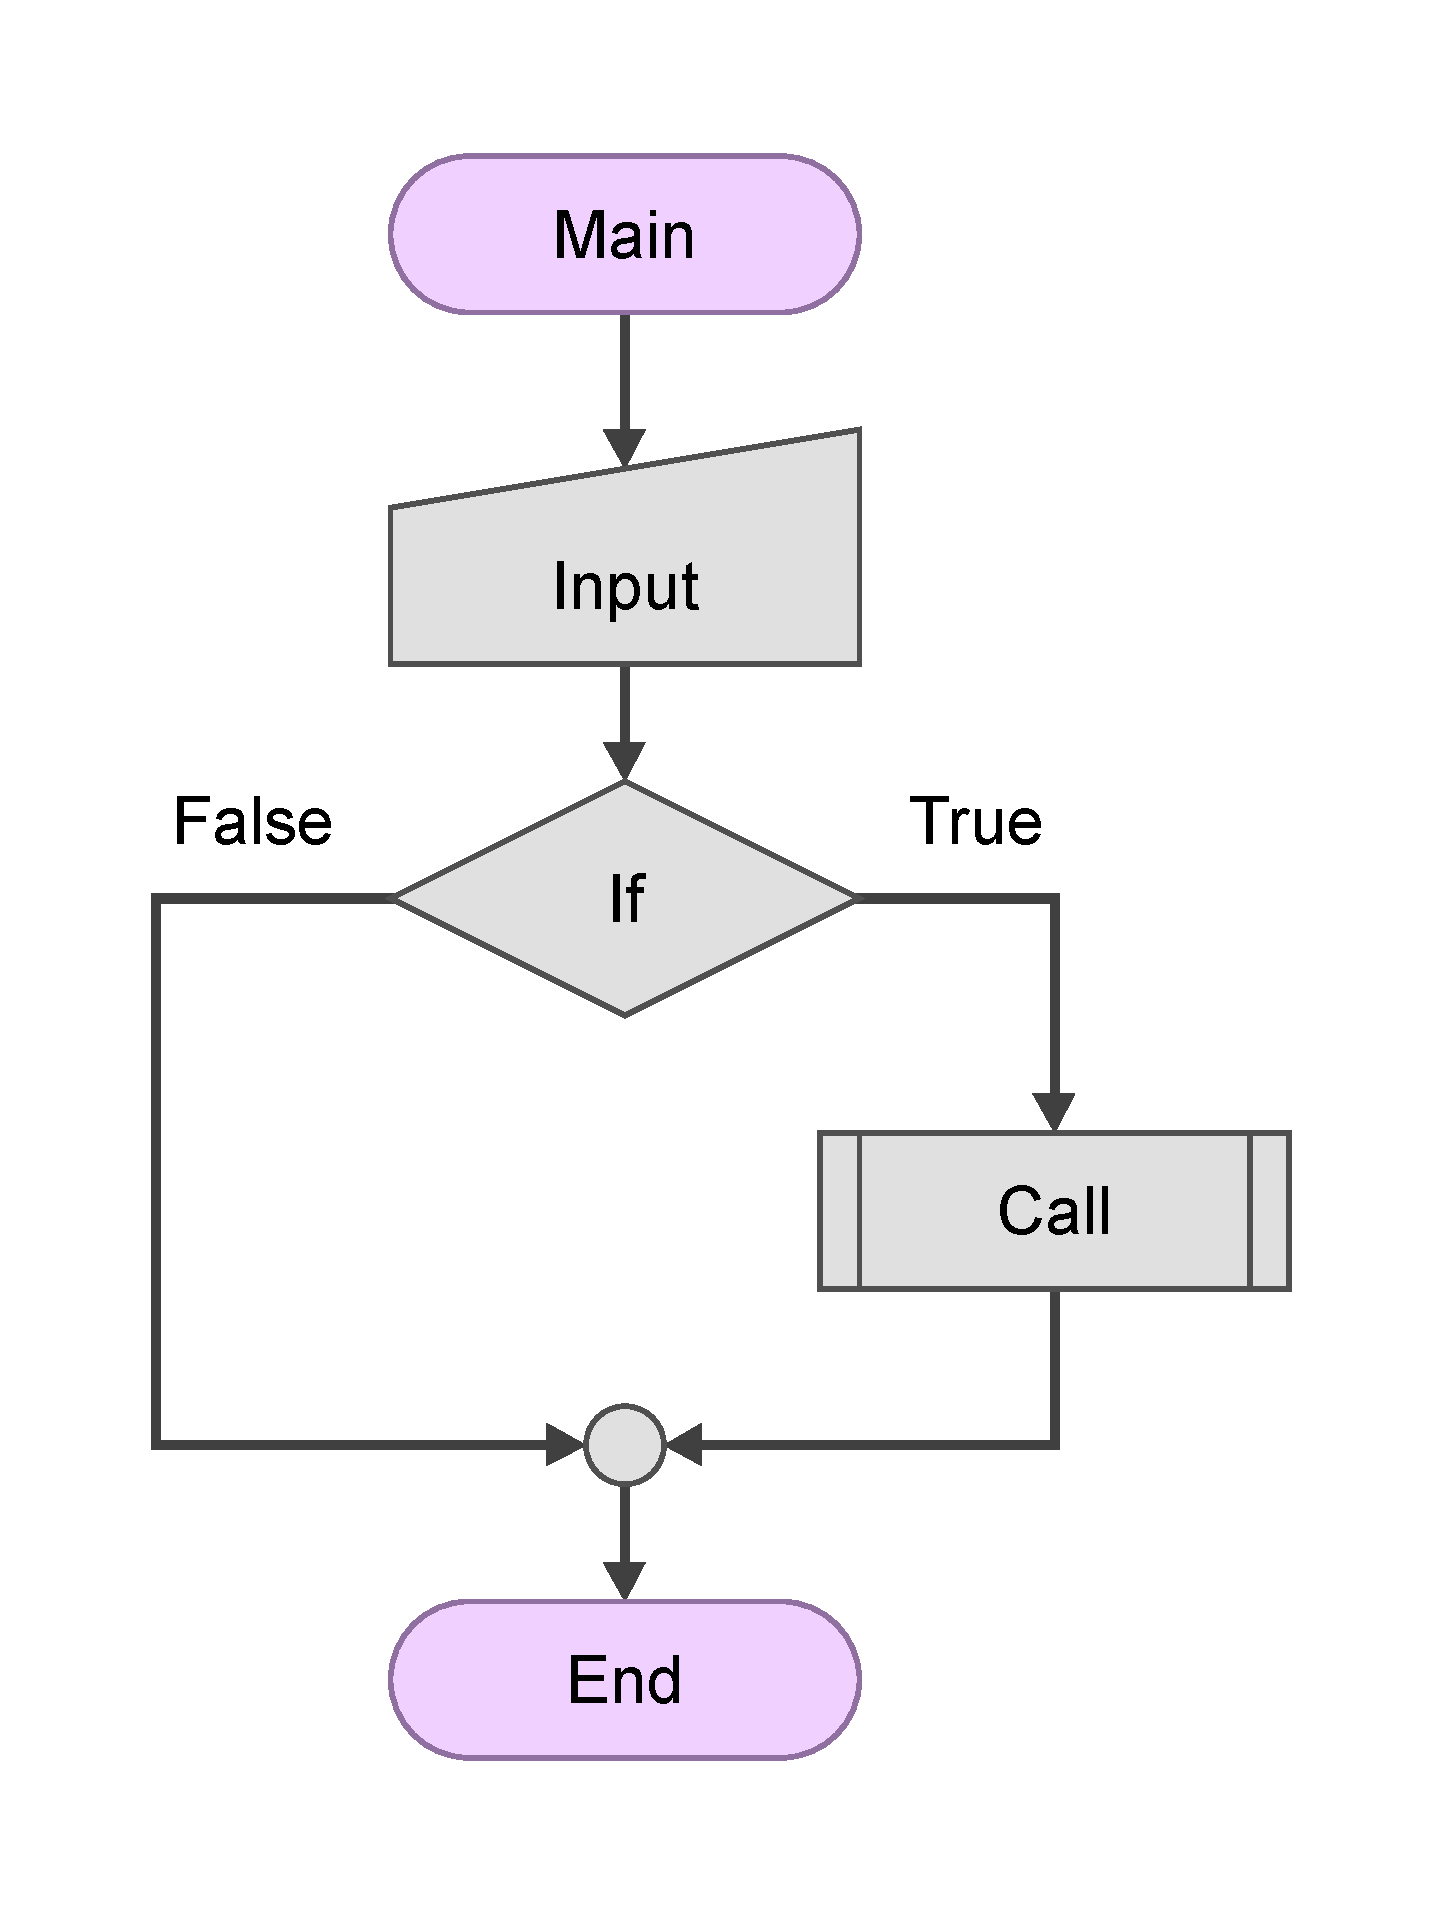
\includegraphics[scale=0.3]{figures/chart.pdf}
    \caption{Example figure in \LaTeX.}
    \label{fig:chart_a}
\end{figure}

\clearpage %  use command \clearpage when you want section or text to appear in the next page.

\section{Example of an algorithm in \LaTeX}
Algorithm~\ref{algo:algo_example} is a good example of an algorithm in \LaTeX.  
\begin{algorithm}
    \caption{Example caption: sum of all even numbers}
    \label{algo:algo_example}
    \begin{algorithmic}[1]
        \Require{$ \mathbf{x}  = x_1, x_2, \ldots, x_N$}
        \Ensure{$EvenSum$ (Sum of even numbers in $ \mathbf{x} $)}
        \Statex
        \Function{EvenSummation}{$\mathbf{x}$}
        \State {$EvenSum$ $\gets$ {$0$}}
        \State {$N$ $\gets$ {$length(\mathbf{x})$}}
        \For{$i \gets 1$ to $N$}                    
        \If{$ x_i\mod 2 == 0$}  \Comment check if a number is even?
        \State {$EvenSum$ $\gets$ {$EvenSum + x_i$}}
        \EndIf
        \EndFor
        \State \Return {$EvenSum$}
        \EndFunction
    \end{algorithmic}
\end{algorithm}
 
\section{Example of code snippet  in \LaTeX}

Code Listing~\ref{list:python_code_ex} is a good example of including a code snippet in a report. While using code snippets, take care of the following:
\begin{itemize}
    \item do not paste your entire code (implementation) or everything you have coded. Add code snippets only. 
    \item The algorithm shown in Algorithm~\ref{algo:algo_example} is usually preferred over code snippets in a technical/scientific report. 
    \item Make sure the entire code snippet or algorithm stays on a single page and does not overflow to another page(s).  
\end{itemize}

Here are three examples of code snippets for three different languages (Python, Java, and CPP) illustrated in Listings~\ref{list:python_code_ex}, \ref{list:java_code_ex}, and \ref{list:cpp_code_ex} respectively.  

\begin{lstlisting}[language=Python, caption={Code snippet in \LaTeX ~and  this is a Python code example}, label=list:python_code_ex]
import numpy as np

x  = [0, 1, 2, 3, 4, 5] # assign values to an array
evenSum = evenSummation(x) # call a function

def evenSummation(x):
    evenSum = 0
    n = len(x)
    for i in range(n):
        if np.mod(x[i],2) == 0: # check if a number is even?
            evenSum = evenSum + x[i]
    return evenSum
\end{lstlisting}

Here we used  the ``\textbackslash clearpage'' command and forced-out the second listing example onto the next page. 
\clearpage  %
\begin{lstlisting}[language=Java, caption={Code snippet in \LaTeX ~and  this is a Java code example}, label=list:java_code_ex]
public class EvenSum{ 
    public static int evenSummation(int[] x){
        int evenSum = 0;
        int n = x.length;
        for(int i = 0; i < n; i++){
            if(x[i]%2 == 0){ // check if a number is even?
                evenSum = evenSum + x[i];
            }
        }
        return evenSum;     
    }
    public static void main(String[] args){ 
        int[] x  = {0, 1, 2, 3, 4, 5}; // assign values to an array
        int evenSum = evenSummation(x);
        System.out.println(evenSum);
    } 
} 
\end{lstlisting}


\begin{lstlisting}[language=C, caption={Code snippet in \LaTeX ~and  this is a C/C++ code example}, label=list:cpp_code_ex]
int evenSummation(int x[]){
    int evenSum = 0;
    int n = sizeof(x);
    for(int i = 0; i < n; i++){
        if(x[i]%2 == 0){ // check if a number is even?
            evenSum = evenSum + x[i];
    	}
    }
    return evenSum;     
}

int main(){
    int x[]  = {0, 1, 2, 3, 4, 5}; // assign values to an array
    int evenSum = evenSummation(x);
    cout<<evenSum;
    return 0;
}
\end{lstlisting}



\section{Example of in-text citation style}
\subsection{Example of the equations and illustrations placement and reference in the text}
Make sure whenever you refer to the equations, tables, figures, algorithms,  and listings for the first time, they also appear (placed) somewhere on the same page or in the following page(s). Always make sure to refer to the equations, tables and figures used in the report. Do not leave them without an \textbf{in-text citation}. You can refer to equations, tables and figures more them once.

\subsection{Example of the equations and illustrations style}
Write \textbf{Eq.} with an uppercase ``Eq`` for an equation before using an equation number with (\textbackslash eqref\{.\}). Use ``Table'' to refer to a table, ``Figure'' to refer to a figure, ``Algorithm'' to refer to an algorithm and ``Listing'' to refer to listings (code snippets). Note that, we do not use the articles ``a,'' ``an,'' and ``the'' before the words Eq., Figure, Table, and Listing, but you may use an article for referring the words figure, table, etc. in general.

For example, the sentence ``A report structure is shown in \textbf{the} Table~\ref{tab:gen_template}'' should be written as ``A report structure is shown \textbf{in} Table~\ref{tab:gen_template}.'' 
 

\section{Summary}
Write a summary of this chapter.

~\\[5em]
\noindent
{\huge\textbf{Note:}} In the case of \textbf{software engineering} project a Chapter ``\textbf{Testing and Validation}'' should precede the ``Results'' chapter. See Section~\ref{subsec:se_chpters} for report organization of such project. 


    \chapter{Results}
\label{ch:results}
The results chapter tells a reader about your findings based on the methodology you have used to solve the investigated problem. For example: 
\begin{itemize}
    \item If your project aims to develop a software/web application, the results may be the developed software/system/performance of the system, etc., obtained using a relevant methodological approach in software engineering. 
    
    \item If your project aims to implement an algorithm for its analysis, the results may be the performance of the algorithm obtained using a relevant experiment design. 
    
    \item If your project aims to solve some problems/research questions over a collected dataset, the results may be the findings obtained using the applied tools/algorithms/etc. 
\end{itemize}
Arrange your results and findings in a logical sequence. 



\section{A section}

...

\clearpage
\section{Example of a Table in \LaTeX}
Table~\ref{tab:_ex_tab} is an example of a table created using the package \LaTeX  ``booktabs.'' do check the link: \href{https://en.wikibooks.org/wiki/LaTeX/Tables}{wikibooks.org/wiki/LaTeX/Tables} for more details. A table should be clean and readable. Unnecessary horizontal lines and vertical lines in tables make them unreadable and messy. The example in Table~\ref{tab:_ex_tab} uses a minimum number of liens (only necessary ones). Make sure that the top rule and bottom rule (top and bottom horizontal lines) of a table are present. 

\begin{table}[h!]
    \centering
    \caption{Example of a table in \LaTeX}
    \label{tab:_ex_tab}
    \begin{tabular}{llr}     
        \toprule
        \multicolumn{2}{c}{Bike} \\
        \cmidrule(r){1-2}
        Type    &  Color & Price (\pounds) \\
        \midrule
        Electric    & black   & 700   \\
        Hybrid      & blue    & 500   \\
        Road        & blue    & 300   \\
        Mountain    & red     & 300   \\
        Folding     & black   & 500   \\
        \bottomrule
    \end{tabular}
\end{table}

\section{Example of captions style}

\begin{itemize}
    \item The \textbf{caption of a Figure (artwork) goes below} the artwork (Figure/Graphics/illustration). See example artwork in Figure~\ref{fig:chart_a}. 
    \item  The \textbf{caption of a Table goes above} the table. See the example in Table~\ref{tab:_ex_tab}.
    \item  The \textbf{caption of an Algorithm goes above} the algorithm. See the example in Algorithm~\ref{algo:algo_example}.
    \item The \textbf{caption of a Listing goes below} the Listing  (Code snippet). See example listing in Listing~\ref{list:python_code_ex}. 
\end{itemize} 





\section{Summary}
Write a summary of this chapter.




    \chapter{Discussion and Analysis}
\label{ch:evaluation}

Depending on the type of project you are doing, this chapter can be merged with ``Results'' Chapter as `` Results and Discussion'' as suggested by your supervisor. 

In the case of software development and the standalone applications, describe the significance of the obtained results/performance of the system. 



\section{A section}% please use an appropriate section title
Discussion and analysis chapter evaluates and analyses the results. It interprets the obtained results. 



\section{Significance of the findings}
In this chapter, you should also try to discuss the significance of the results and key findings, in order to enhance the reader's understanding of the investigated problem

\section{Limitations} % please discuss limitation of the project 
Discuss the key limitations and potential implications or improvements of the findings.
\section{Summary}
Write a summary of this chapter.
    \chapter{Conclusions and Future Work}
\label{ch:con}
\section{Conclusions}
Typically a conclusions chapter first summarizes the investigated problem and its aims and objectives. It summaries the critical/significant/major findings/results about the aims and objectives that have been obtained by applying the key methods/implementations/experiment set-ups. A conclusions chapter draws a picture/outline of your project's central and the most signification contributions and achievements. 

A good conclusions summary could be approximately 300--500 words long, but this is just a recommendation.

A conclusions chapter followed by an abstract is the last things you write in your project report.

\section{Future work}
This section should refer to Chapter~\ref{ch:results} where the author has reflected their criticality about their own solution. The future work is then sensibly proposed in this section.

\textbf{Guidance on writing future work:} While working on a project, you gain experience and learn the potential of your project and its future works. Discuss the future work of the project in technical terms. This has to be based on what has not been yet achieved in comparison to what you had initially planned and what you have learned from the project. Describe to a reader what future work(s) can be started from the things you have completed. This includes identifying what has not been achieved and what could be achieved. 



A good future work summary could be approximately 300--500 words long, but this is just a recommendation.
    \chapter{Reflection}
\label{ch:reflection}
%%%%%%%%%%%%%%%%%%%%%%%%%%%%%%%
%% Please remove/replace text below
%%%%%%%%%%%%%%%%%%%%%%%%%%%%%%%
Write a short paragraph on the substantial learning experience. This can include your decision-making approach in problem-solving.

\textbf{Some hints:} You obviously learned how to use different programming languages, write reports in \LaTeX and use other technical tools. In this section, we are more interested in what you thought about the experience. Take some time to think and reflect on your individual project as an experience, rather than just a list of technical skills and knowledge. You may describe things you have learned from the research approach and strategy, the process of identifying and solving a problem, the process research inquiry, and the understanding of the impact of the project on your learning experience and future work.

Also think in terms of:
\begin{itemize}
    \item what knowledge and skills you have developed
    \item what challenges you faced, but was not able to overcome
    \item what you could do this project differently if the same or similar problem would come
    \item rationalize the divisions from your initial planed aims and objectives.
\end{itemize}


A good reflective summary could be approximately 300--500 words long, but this is just a recommendation.

~\\[2em]
\noindent
{\huge \textbf{Note:}} The next chapter is ``\textbf{References},'' which will be automatically generated if you are using BibTeX referencing method. This template uses BibTeX referencing.  Also, note that there is difference between ``References'' and ``Bibliography.'' The list of ``References'' strictly only contain the list of articles, paper, and content you have cited (i.e., refereed) in the report. Whereas Bibliography is a list that contains the list of articles, paper, and content you have cited in the report plus the list of articles, paper, and content you have read in order to gain knowledge from. We recommend to use only the list of ``References.'' 

    

    
    % -------------------------------------------------------------------
    % Bibliography/References  -  Harvard Style was used in this report
    % -------------------------------------------------------------------
    \bibliographystyle{agsm} % Harvard Style 
    
    \bibliography{references}  %  Patashnik, O. (1988), BibTEXing. Documentation for general BibTEX users.
    
    % -------------------------------------------------------------------
    % Appendices
    % -------------------------------------------------------------------
    
    \begin{appendices}
        \chapter{An Appendix Chapter (Optional)}
\label{appn:A}
% Optional chapter
Some lengthy tables, codes, raw data, length proofs, etc. which are \textbf{very important but not essential part} of the project report goes into an Appendix. An appendix is something a reader would consult if he/she needs extra information and a more comprehensive understating of the report. Also, note that you should use one appendix for one idea.

An appendix is optional. If you feel you do not need to include an appendix in your report, avoid including it. Sometime including irrelevant and unnecessary materials in the Appendices may unreasonably increase the total number of pages in your report and distract the reader.


        \chapter{An Appendix Chapter (Optional)}
\label{appn:B}

...
   \end{appendices}
    
\end{document}
